\subsection{UC28 - Suddivisione della planimetria}
\begin{figure}[H]
  \centering
  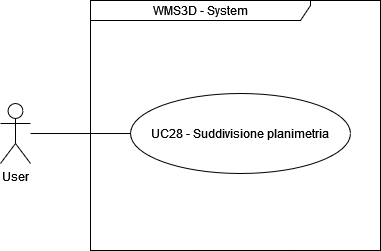
\includegraphics[width=0.5\textwidth]{UC_diagrams_28-32/UC28_sys.drawio.png}
  \caption{Diagramma UML UC28 - Suddivisione della planimetria}
\end{figure}
\begin{figure}[H]
  \centering
  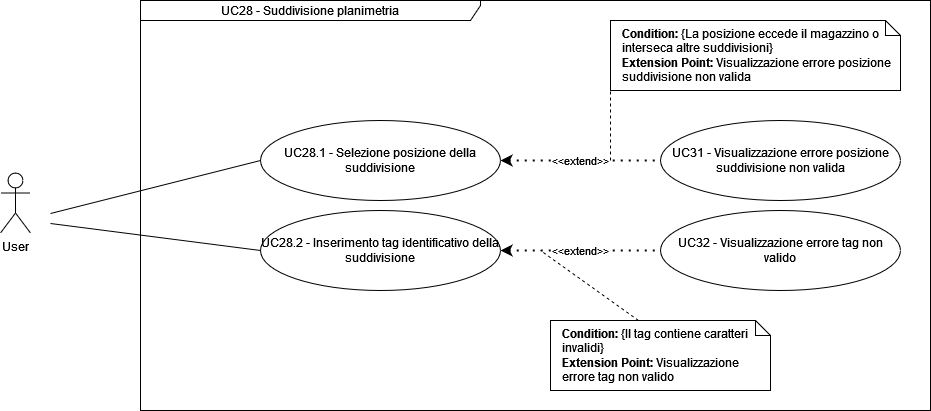
\includegraphics[width=0.9\textwidth]{UC_diagrams_28-32/UC28.drawio.png}
  \caption{Diagramma UML in dettaglio UC28 - Suddivisione della planimetria}
\end{figure}
\begin{itemize}
    \item \textbf{Attori:} User.
    \item \textbf{Pre-condizione:} Il sistema è avviato e funzionante e l’utente ha scelto la planimetria del magazzino [UC1.2.1].
    \item \textbf{Post-condizione:} L'utente ha effettuato una modifica alla suddivisione del magazzino, aggiungendo una nuova area ad esso.
    \item \textbf{Scenario Principale:} L'utente aggiunge una suddivisione al magazzino, scegliendone la posizione [UC28.1] e il tag identificativo [UC28.2]. Le suddivisioni dividono il magazzino in aree specifiche per scopo.
    \item \textbf{Generalizzazioni:} -
    \item \textbf{Estensioni:} -
\end{itemize}

\subsubsection{UC28.1 - Selezione posizione della suddivisione}
\begin{itemize}
    \item \textbf{Attori:} User.
    \item \textbf{Pre-condizione:} Il sistema è avviato e funzionante e l’utente ha scelto la planimetria del magazzino [UC1.2.1]. L'utente ha scelto di inserire una nuova suddivisione della planimetria.
    \item \textbf{Post-condizione:} L'utente ha inserito la posizione della nuova suddivisione.
    \item \textbf{Scenario Principale:} L'utente sceglie una posizione per la nuova suddivisione all'interno della planimetria.
    \item \textbf{Generalizzazioni:} -
    \item \textbf{Estensioni:} È presente una estensione:
        \begin{itemize}
            \item UC31 - Visualizzazione errore posizione suddivisione non valida.
        \end{itemize}
\end{itemize}

\subsubsection{UC28.2 - Inserimento tag identificativo della suddivisione}
\begin{itemize}
    \item \textbf{Attori:} User.
    \item \textbf{Pre-condizione:} Il sistema è avviato e funzionante e l’utente ha scelto la planimetria del magazzino [UC1.2.1]. L'utente ha scelto di inserire una nuova suddivisione della planimetria.
    \item \textbf{Post-condizione:} L'utente ha inserito correttamente un tag per la suddivisione da creare.
    \item \textbf{Scenario Principale:} L'utente sceglie un nome, il cosiddetto tag, per la nuova suddivisione.
    \item \textbf{Generalizzazioni:} -
    \item \textbf{Estensioni:} È presente una estensione:
        \begin{itemize}
            \item UC32 - Visualizzazione errore tag non valido.
        \end{itemize}
\end{itemize}